

\documentclass[color=usenames,dvipsnames]{beamer}

\usepackage[adobefonts,noindent]{ctex} %中文支持
\setCJKmainfont{SimSun}

\mode<presentation> {

\usetheme{Madrid}
\usecolortheme{lily}
\useoutertheme{infolines}

}


\usepackage{booktabs} 
\usepackage{tikz}


\newcommand{\red}[1]{\textcolor{red}{#1}}
\newcommand{\brown}[1]{\textcolor{brown}{#1}}
\newcommand{\green}[1]{\textcolor{green}{#1}}
\newcommand{\blue}[1]{\textcolor{blue}{#1}}
\newcommand{\cyan}[1]{\textcolor{cyan}{#1}}

% Thin fonts
\usepackage{cmbright}
\usepackage[T1]{fontenc}

\definecolor{dark_grey}{gray}{0.5}
\setbeamercolor{normal text}{fg=dark_grey,bg=white}
\setbeamertemplate{navigation symbols}{}

\setbeamercolor*{palette primary}{fg=gray!100,bg=gray!10}
\setbeamercolor*{palette quaternary}{fg=gray!100,bg=gray!10}
\setbeamercolor*{palette secondary}{fg=gray!100,bg=gray!20}
\setbeamercolor*{palette tertiary}{fg=gray!100,bg=gray!10}
\setbeamercolor*{navigation symbols}{fg=white,bg=white}
\usefonttheme{default}


\setbeamertemplate{blocks}[rounded][shadow=false]
\setbeamercolor{block title}{bg=gray!10}
\setbeamercolor{block body}{fg=gray,bg=gray!10}
%\setbeamercolor{frametitle}{fg=}

\setbeamertemplate{frametitle}[default][center]

\setbeamertemplate{itemize items}[default]
\setbeamertemplate{enumerate items}[default]

\newcommand{\F}{\mathbb{F}}


\title[Text+WordNet Embed]{Single or Multiple? Combining Word Representations Independently Learned from Text and WordNet\vspace{0.2cm}}
\subtitle{AAAI 2016}
\author[韩喆]{Josu Goikoetxea, Eneko Agirre, and Aitor Soroa}
\institute[ICSTWIP]{巴斯克大学}
\date[20160308]{}
\begin{document}


\begin{frame}
  \titlepage
\end{frame}

% Uncomment these lines for an automatically generated outline.
%\begin{frame}{Outline}
%  \tableofcontents
%\end{frame}

\begin{frame}{outline}
 \begin{itemize}
  \item 作者简介
  \item 论文简介
  \item 相关工作:transH, retrofitting 
  \item 词向量的生成与合并(random walk)
  \item 实验效果、对比、多组词向量合并效果
 \end{itemize}
\end{frame}

\begin{frame}{作者简介}\footnotesize
  \begin{columns}
   \column{0.45\hsize}
     \begin{block}{}
   \begin{center}
     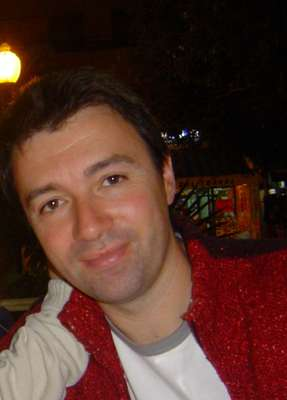
\includegraphics[width=0.35\hsize]{pic/EnekoAgirre.jpg}
   \end{center}
      \begin{itemize}
       \item \href{http://ixa2.si.ehu.es/eneko/}{Eneko Agirre}
       \item Processing of Basque, 语义相似度/关联度,WSD,SRL,IE,。。。
       \item 比较厉害
      \end{itemize}
     \end{block}

     
   \column{0.45\hsize}
   \begin{center}
   \end{center}
     \begin{block}{}
      \begin{itemize}
       \item Josu Goikoetxea
      \end{itemize}
     \end{block}
     
     \begin{block}{}
   \begin{center}
     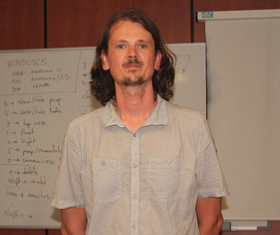
\includegraphics[width=0.55\hsize]{pic/aitor-soroa.png}
   \end{center}
      \begin{itemize}
       \item Aitor Soroa
       \item NLP,CL,AI
      \end{itemize}
     \end{block}
  \end{columns}

\end{frame}


\frame{
  \begin{columns}[c]
   \column{.15\hsize}
   \column{.7\hsize}
   \begin{block}{}
    \centering \Large 论文简介  \\ 
   \end{block}
   \column{.15\hsize}
  \end{columns}
}

\frame{
  \frametitle{论文简介}
  
  \begin{block}{我有很多不同类型的语料,怎么训练出一个好的词向量?}
   \pause
   \red{直接在不同的语料上跑word2vec, 然后把这些词向量拼接起来/PCA就好了!}
  \end{block} 
}


\frame{
  \begin{columns}[c]
   \column{.15\hsize}
   \column{.7\hsize}
   \begin{block}{}
    \centering \Large 相关工作  \\ 
    \small --- 不同的语料注入到一个词向量 \\ 
   \end{block}
   \column{.15\hsize}
  \end{columns}
}

\frame{
  \frametitle{相关工作}
  \begin{columns}[c]
   \column{0.45\hsize}
  \begin{block}{2012.SIGKDD}
    将WordNet的信息加入目标函数中训练,要求WordNet中有关联的点词向量近
  \end{block}

  \begin{block}{2014.AAAI transH}
    \begin{center}
     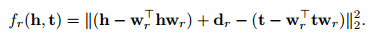
\includegraphics[width=0.97\hsize]{pic/transHgs.png}\\ 
     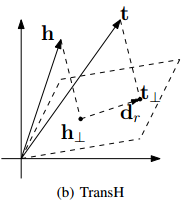
\includegraphics[width=0.6\hsize]{pic/transH.png}
    \end{center}
  \end{block}
  
   \column{0.5\hsize}
  \begin{block}{2014.EACL }
   将不同语言的词向量映射到同一个平面,然后使用\href{http://www.cnblogs.com/jerrylead/archive/2011/06/20/2085491.html}{CCA}找到关联,将不同语言的词向量通过不同的矩阵映射到同一个空间
    \begin{center}
     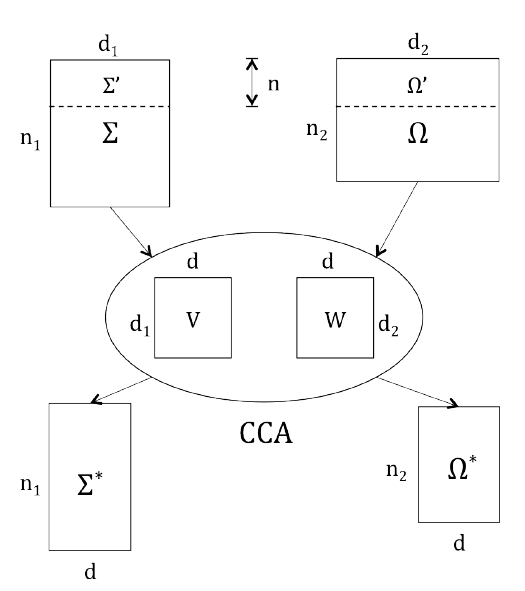
\includegraphics[width=0.6\hsize]{pic/eacl2014.png}
    \end{center}
  \end{block}
  \end{columns}
}

\frame{
  \frametitle{相关工作}
  \begin{block}{2015.EMNLP Retrofitting with Semantic Lexicons-\red{顺序模型}}
  \begin{columns}[c]
   \column{0.43\hsize}
      \vspace{2mm}
      \centering 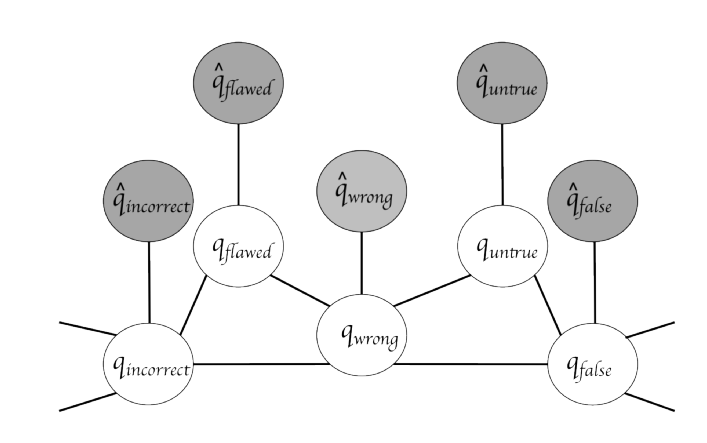
\includegraphics[width=0.98\hsize]{pic/retrofit.png}
      
    \column{0.55\hsize}
      \begin{enumerate}
       \item 传统工具(word2vec)生成初始向量空间$\hat{Q}$ (左图灰色点)
       \item 根据语义字典生成$\Omega$ (左图的边)
       \item 最优(小)化 $\Psi(Q)=$\\  
      \vspace{3mm}
      \end{enumerate}
       \small $\sum_{i=1}^n\biggl[\alpha_i\big\|q_i-\hat{q_i}\big\|^2+\sum_{(i,j)\in E}\beta_{ij}\big\|q_i-q_j\big\|^2\biggl]$
  \end{columns}
  \end{block}

  \begin{block}{2015.NACCL Multiview LSA: Representation Learning via Generalized CCA}
   使用Generalized CCA 将Wikipedia,PPDB,WordNet,FrameNet,CatVar生成的不同的词向量合并成一个向量
  \end{block}
}


\frame{
  \begin{columns}[c]
   \column{.15\hsize}
   \column{.7\hsize}
   \begin{block}{}
    \centering \Large 实验方法  \\ 
    \small --- 词向量生成 \\ 
    \small --- 词向量合并 \\ 
   \end{block}
   \column{.15\hsize}
  \end{columns}
}

\frame{
  \frametitle{实验方法.词向量生成}
  \begin{block}{从text生成的词向量}
   (Wikipedia+British National Corpus+ukWaC)+word2vec.skipgram
  \end{block}

  \begin{block}{从WordNet(WN)生成的词向量}
   \begin{enumerate}
    \item 在WN上做random walk,得到一些路径,每条路径就是一个“句子”
      \begin{itemize}
       \item 一个例子:yucatec(尤卡坦语) mayan quiche(火腿起司蛋卷) kekchi(克奇人) speak sino-tibetan(汉藏语系) tone language west chadic(乍得) talk
      \end{itemize}

    \item 对这些“句子”生成的“假文本”+word2vec.skipgram得到向量
   \end{enumerate}
  \end{block}
}

\frame{
  \frametitle{random walk(RW)}
  \begin{itemize}
   \item random walk = 双向 path ranking algorithm (PRA) + sampling \\ 
  \end{itemize}
  \begin{columns}[c]
   \column{0.5\hsize}
  \centering 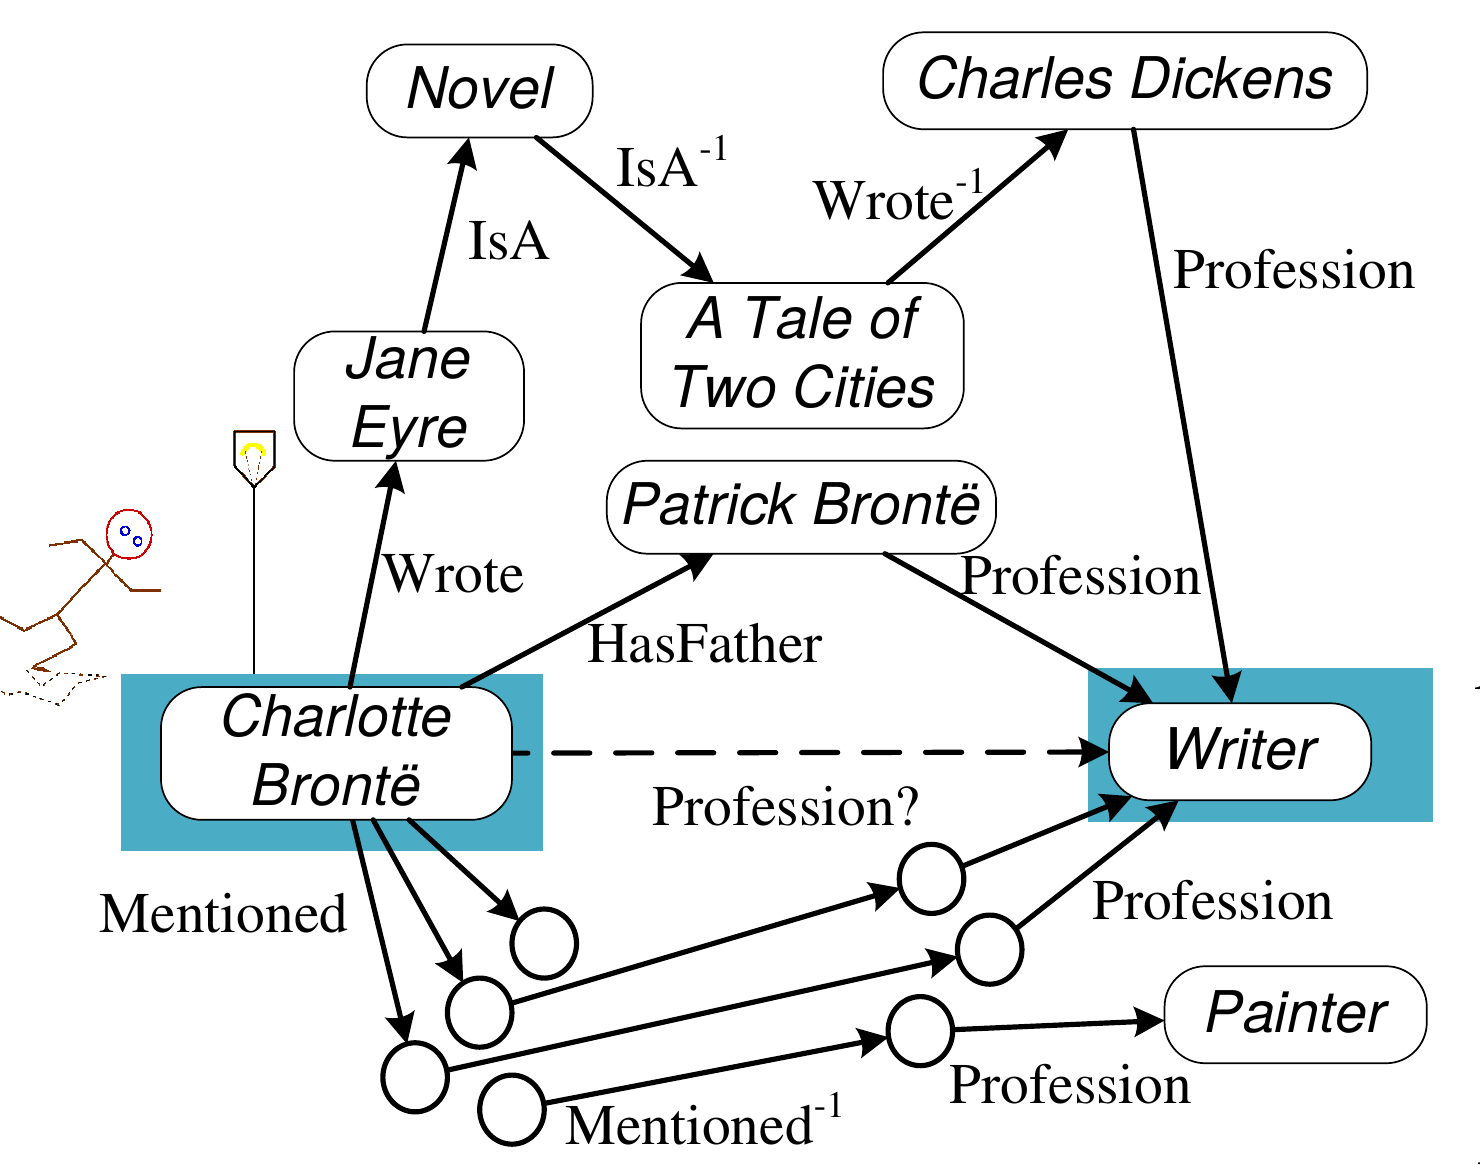
\includegraphics[width=0.95\hsize]{pic/pra.png}
   \column{0.5\hsize}
  \centering 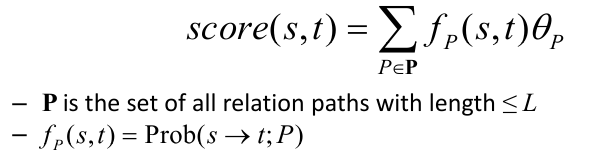
\includegraphics[width=0.98\hsize]{pic/PRAgs.png} \\ 
  \end{columns}
}

\frame{
  \frametitle{实验方法.词向量合并-1}
  \begin{block}{词向量直接组合}
   \begin{enumerate}
    \item CAT(concatenating): 2个词向量拼接(300维->600维)
    \item CEN(centroid): 词向量平均
    \item CMP(complex):组合成一个复数,($v_1+v_2i$)
   \end{enumerate}
  \end{block}
  
  \begin{block}{相关性分析}
   \begin{enumerate}
    \item PCA: CAT->300维
    \item CCA: 将2个词向量映射到一个新的、一致的向量空间
   \end{enumerate}
  \end{block}
  
  \begin{block}{语料组合}
   (Wikipedia+British National Corpus+ukWaC+\red{\textbf{random walk生成的“假文本”}})+word2vec.skipgram
  \end{block}
}

\frame{
  \frametitle{实验方法.词向量合并-2}
  \begin{block}{相似度组合}
   \begin{enumerate}
     \item AVG: 不合并2组向量,计算相似度的时候使用2个相似度的均值
     \item RNK: 对于每组向量:对于实验中的数据计算相似度并排序。用2个排名的平均值作为每组数据的最终排名
    \end{enumerate}
  \end{block}
  

  \pause
  
  \vspace{2mm}
  评价结果好坏采用斯皮尔曼等级相关系数
  \vspace{1mm}
  
  \begin{columns}[c]
   \column{0.6\hsize}
   \centering 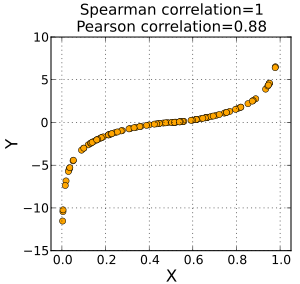
\includegraphics[width=0.5\hsize]{pic/Spearman.png}
   \centering 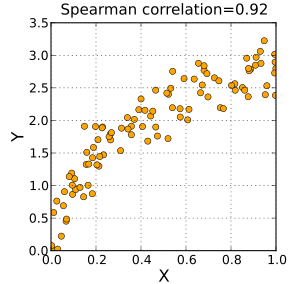
\includegraphics[width=0.5\hsize]{pic/Spearman2.png}
   \column{0.45\hsize}
   $\rho=\frac{\sum_i(x_i-\bar{x})(y_i-\bar{y})}{\sqrt{\sum_i(x_i-\bar{x})^2\sum_i(y_i-\bar{y})^2}}\in [-1,1]$
  \end{columns}
}


\frame{
  \begin{columns}[c]
   \column{.15\hsize}
   \column{.7\hsize}
   \begin{block}{}
    \centering \Large 实验  \\ 
    \small --- 0. 数据集
    \small --- 1. 不同词向量组合的效果 \\ 
    \small --- 2. 和NACCL2015 Retrofitting 的对比 \\ 
    \small --- 3. 简单对比其他的词向量组合/提升模型 \\ 
    \small --- 4. 多种(>2)语料的词向量混合 \\ 
   \end{block}
   \column{.15\hsize}
  \end{columns}
}

\frame{
  \frametitle{实验.数据集}
  
  \begin{columns}[c]
   \column{0.46\hsize}
  \begin{block}{WordSim353 Similarity(WSS)}
   \begin{itemize}\begin{footnotesize}
    \item 353个英语单词对(200个13个人标,153个16个人标),相似度:0-10
    \item 定义:Word 1	Word 2	Human (mean)
    \item 例子:love	sex	6.77
    \end{footnotesize}
   \end{itemize}
  \end{block}
  \begin{block}{RG-65(RG)}
  \end{block}
  \begin{block}{MTURK287(MTU)}
  \end{block}
   
   \column{0.52\hsize}
  \begin{block}{WordSim353 Relatedness(WSR)}
   \begin{itemize}\begin{footnotesize}
    \item 252个英语单词对,相关度:0-10
    \item 定义:Word 1	Word 2	Human (mean)
    \item 例子:planet	galaxy	8.11
    \end{footnotesize}
   \end{itemize}
  \end{block}
  
  \begin{block}{MEN}
   \begin{itemize}
    \item 3000对单词(共现700次)
   \end{itemize}
  \end{block}
   
  \end{columns}
  
  \begin{block}{SimLex-999(SL)}
      \begin{itemize}\begin{footnotesize}
       \item 999对相同词性的单词对,0-10的相似度(0表示完全不相似)
       \item 数据格式:word1	word2	POS	SimLex999	conc(w1)	conc(w2)	concQ	Assoc(USF)...
       \item 例子:smart	intelligent	A	9.2	1.75	2.46	1	7.11	...
    \end{footnotesize}
      \end{itemize}
  \end{block}
 
}

\frame{
  \frametitle{实验.不同词向量组合的效果}
  \begin{center}
    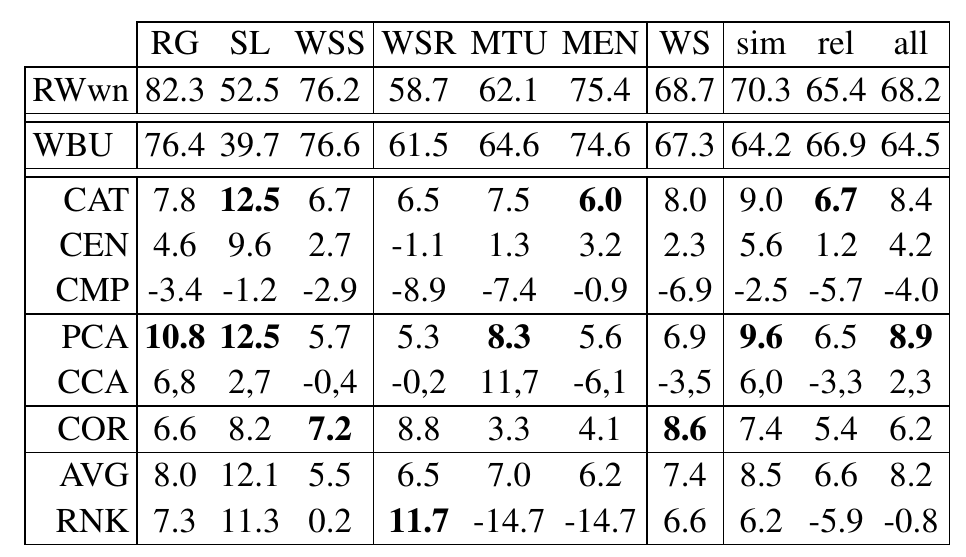
\includegraphics[width=0.8\hsize]{pic/expComb.png}
  \end{center}
  
  \begin{itemize}
   \item CAT:拼接,AVG:相似度均值,COR:语料混合,CEN:向量平均,RNK:相似度排名均值,CMP:复数表示
   \item $PCA>CAT\approx AVG>COR>CEN>CMP$
  \end{itemize}
}

\frame{
  \frametitle{实验.和NACCL2015 Retrofitting 的对比}
  \begin{columns}[c]
   \column{0.7\hsize}
  \begin{center}
    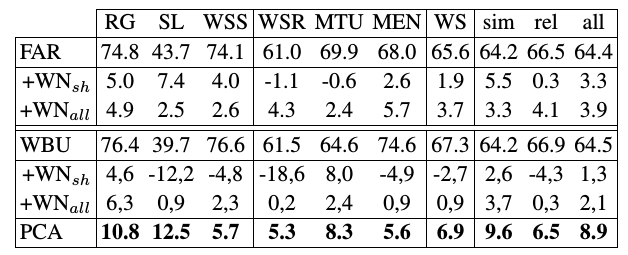
\includegraphics[width=0.99\hsize]{pic/expRetrofit.png}
  \end{center}
   \column{0.3\hsize}
   $WN_{sh}$:上位、同义词 \\ 
   $WN_{all}$:还用“part-of”,“gloss relation”等关系
  \end{columns}

  
  \begin{itemize}
   \item 前三行是原文章的效果,下面4行是本文的效果
   \item 2,3行说明:上位、同义信息对于相似度判断有帮助,WordNet的全部关系对判断单词relation有帮助
   \item 说明作者的WordNet向量还是很有竞争力的
   \item 为什么作者的好:(physics-proton)在WN没有关联边,retrofit作用没效果;但是作者训练出来的WN-vec中却是非常相似的2个向量
   \item 作者实验的缺点:如果把WordNet换成PPPD,作者的实验不能得到提升,反而下降
  \end{itemize}
}

\frame{
  \frametitle{实验.简单对比其他的词向量组合/提升模型}
  \begin{center}
    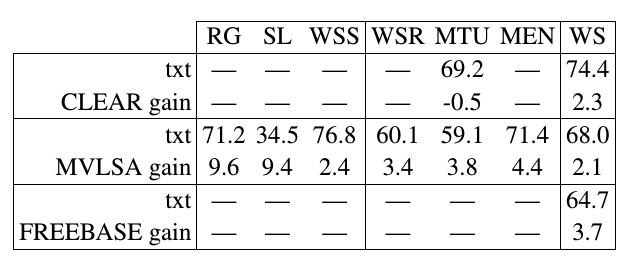
\includegraphics[width=0.6\hsize]{pic/expOther.png}
  \end{center}
  \begin{block}{CLEAR}
   Yahoo! Answers corpus + WordNet上位词、同义词、meronyms(部分名词)
  \end{block}

  
  \begin{columns}[c]
   \column{0.45\hsize}
  \begin{block}{MVLSA}
   LSA+WordNet
  \end{block}
   \column{0.45\hsize}
  \begin{block}{FREEB}
    freebase relation 优化
  \end{block}
  \end{columns}
  
  \begin{itemize}
   \item 本文和上面三个都没有可比性,因为baseline不一样,不过第三个使用Freebase的信息引导作者从Wikipedia上面挖更多的语料
  \end{itemize}


  
}
\frame{
  \frametitle{实验.多种(>2)语料的词向量混合}
  \begin{columns}[c]
   \column{0.6\hsize}
  \begin{center}
    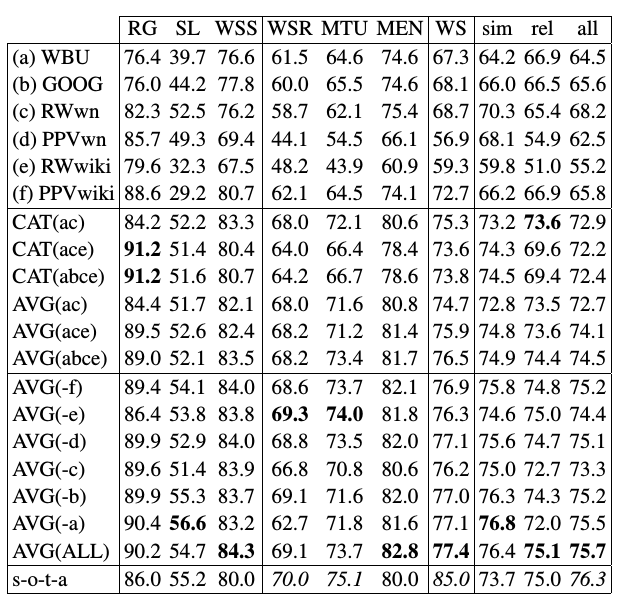
\includegraphics[width=0.99\hsize]{pic/expMulti.png}
  \end{center}
  
   \column{0.4\hsize}
    \begin{block}{6种语料/词向量}
     \begin{enumerate}\begin{footnotesize}
      \item WBU: 之前的文本语料
      \item GOOG: google news训练好的
      \item \cyan{RWwn}: 之前的“伪语料
      \item \red{PPVwn}: 在WrodNet上使用Personalized PageRank得到
      \item \cyan{RWwiki}: 在维基百科页面上仿照WordNet做Random walk 生成语料。2个页面之间有超链接则相连
      \item \red{PPVwiki}: 在Wikipedia上使用 Personalized PageRank得到
      \end{footnotesize}
     \end{enumerate}
    \end{block}
  \end{columns}

  \begin{itemize}
   \item CAT 对于超过2个来源就不管用了;“-1”实验说明每个语料都有用
  \end{itemize}
}

\frame{
  \frametitle{总结}
  \begin{itemize}
   \item 简单的词向量拼接就很不错了
   \item 对于WordNet 这样的资源,在上面训练一个还不错的词向量要比把WordNet的信息嵌入到文本训练中更有用
  \end{itemize}
}

\frame{
  \begin{columns}[c]
   \column{.2\hsize}
   \column{.6\hsize}
   \begin{block}{}
   \vspace{0.4cm}
    \centering \Large 问题?  \\ 
   \vspace{0.4cm}
   \end{block}
   \column{.2\hsize}
  \end{columns}
}


\frame{
  \frametitle{我的问题}
  \begin{enumerate}
   \item AVG 和 CEN 不是一样的吗?
   \pause
   \item 对于WordNet的信息,下面两个数据用word2vec训练哪个效果好?
   \begin{columns}[c]
    \column{0.47\hsize}
    \begin{block}{窗口大小5}
      \begin{itemize}
       \item yucatec mayan quiche kekchi
       \item speak sino-tibetan tone language west chadic talk
      \end{itemize}
    \end{block}

    \column{0.46\hsize}
      \begin{block}{窗口大小1或2}
      \begin{itemize}
       \item s yucatec WN-synonymy mayan e
       \item s mayan WN-category quiche e
       \item s quiche WN-category-rev kekchi e
       \item ...
      \end{itemize}
      \end{block}
   \end{columns}

  \end{enumerate}

}


\end{document} 